% Options for packages loaded elsewhere
\PassOptionsToPackage{unicode}{hyperref}
\PassOptionsToPackage{hyphens}{url}
%
\documentclass[
]{article}
\usepackage{lmodern}
\usepackage{amssymb,amsmath}
\usepackage{ifxetex,ifluatex}
\ifnum 0\ifxetex 1\fi\ifluatex 1\fi=0 % if pdftex
  \usepackage[T1]{fontenc}
  \usepackage[utf8]{inputenc}
  \usepackage{textcomp} % provide euro and other symbols
\else % if luatex or xetex
  \usepackage{unicode-math}
  \defaultfontfeatures{Scale=MatchLowercase}
  \defaultfontfeatures[\rmfamily]{Ligatures=TeX,Scale=1}
\fi
% Use upquote if available, for straight quotes in verbatim environments
\IfFileExists{upquote.sty}{\usepackage{upquote}}{}
\IfFileExists{microtype.sty}{% use microtype if available
  \usepackage[]{microtype}
  \UseMicrotypeSet[protrusion]{basicmath} % disable protrusion for tt fonts
}{}
\makeatletter
\@ifundefined{KOMAClassName}{% if non-KOMA class
  \IfFileExists{parskip.sty}{%
    \usepackage{parskip}
  }{% else
    \setlength{\parindent}{0pt}
    \setlength{\parskip}{6pt plus 2pt minus 1pt}}
}{% if KOMA class
  \KOMAoptions{parskip=half}}
\makeatother
\usepackage{xcolor}
\IfFileExists{xurl.sty}{\usepackage{xurl}}{} % add URL line breaks if available
\IfFileExists{bookmark.sty}{\usepackage{bookmark}}{\usepackage{hyperref}}
\hypersetup{
  hidelinks,
  pdfcreator={LaTeX via pandoc}}
\urlstyle{same} % disable monospaced font for URLs
\usepackage[margin=1in]{geometry}
\usepackage{color}
\usepackage{fancyvrb}
\newcommand{\VerbBar}{|}
\newcommand{\VERB}{\Verb[commandchars=\\\{\}]}
\DefineVerbatimEnvironment{Highlighting}{Verbatim}{commandchars=\\\{\}}
% Add ',fontsize=\small' for more characters per line
\usepackage{framed}
\definecolor{shadecolor}{RGB}{248,248,248}
\newenvironment{Shaded}{\begin{snugshade}}{\end{snugshade}}
\newcommand{\AlertTok}[1]{\textcolor[rgb]{0.94,0.16,0.16}{#1}}
\newcommand{\AnnotationTok}[1]{\textcolor[rgb]{0.56,0.35,0.01}{\textbf{\textit{#1}}}}
\newcommand{\AttributeTok}[1]{\textcolor[rgb]{0.77,0.63,0.00}{#1}}
\newcommand{\BaseNTok}[1]{\textcolor[rgb]{0.00,0.00,0.81}{#1}}
\newcommand{\BuiltInTok}[1]{#1}
\newcommand{\CharTok}[1]{\textcolor[rgb]{0.31,0.60,0.02}{#1}}
\newcommand{\CommentTok}[1]{\textcolor[rgb]{0.56,0.35,0.01}{\textit{#1}}}
\newcommand{\CommentVarTok}[1]{\textcolor[rgb]{0.56,0.35,0.01}{\textbf{\textit{#1}}}}
\newcommand{\ConstantTok}[1]{\textcolor[rgb]{0.00,0.00,0.00}{#1}}
\newcommand{\ControlFlowTok}[1]{\textcolor[rgb]{0.13,0.29,0.53}{\textbf{#1}}}
\newcommand{\DataTypeTok}[1]{\textcolor[rgb]{0.13,0.29,0.53}{#1}}
\newcommand{\DecValTok}[1]{\textcolor[rgb]{0.00,0.00,0.81}{#1}}
\newcommand{\DocumentationTok}[1]{\textcolor[rgb]{0.56,0.35,0.01}{\textbf{\textit{#1}}}}
\newcommand{\ErrorTok}[1]{\textcolor[rgb]{0.64,0.00,0.00}{\textbf{#1}}}
\newcommand{\ExtensionTok}[1]{#1}
\newcommand{\FloatTok}[1]{\textcolor[rgb]{0.00,0.00,0.81}{#1}}
\newcommand{\FunctionTok}[1]{\textcolor[rgb]{0.00,0.00,0.00}{#1}}
\newcommand{\ImportTok}[1]{#1}
\newcommand{\InformationTok}[1]{\textcolor[rgb]{0.56,0.35,0.01}{\textbf{\textit{#1}}}}
\newcommand{\KeywordTok}[1]{\textcolor[rgb]{0.13,0.29,0.53}{\textbf{#1}}}
\newcommand{\NormalTok}[1]{#1}
\newcommand{\OperatorTok}[1]{\textcolor[rgb]{0.81,0.36,0.00}{\textbf{#1}}}
\newcommand{\OtherTok}[1]{\textcolor[rgb]{0.56,0.35,0.01}{#1}}
\newcommand{\PreprocessorTok}[1]{\textcolor[rgb]{0.56,0.35,0.01}{\textit{#1}}}
\newcommand{\RegionMarkerTok}[1]{#1}
\newcommand{\SpecialCharTok}[1]{\textcolor[rgb]{0.00,0.00,0.00}{#1}}
\newcommand{\SpecialStringTok}[1]{\textcolor[rgb]{0.31,0.60,0.02}{#1}}
\newcommand{\StringTok}[1]{\textcolor[rgb]{0.31,0.60,0.02}{#1}}
\newcommand{\VariableTok}[1]{\textcolor[rgb]{0.00,0.00,0.00}{#1}}
\newcommand{\VerbatimStringTok}[1]{\textcolor[rgb]{0.31,0.60,0.02}{#1}}
\newcommand{\WarningTok}[1]{\textcolor[rgb]{0.56,0.35,0.01}{\textbf{\textit{#1}}}}
\usepackage{graphicx,grffile}
\makeatletter
\def\maxwidth{\ifdim\Gin@nat@width>\linewidth\linewidth\else\Gin@nat@width\fi}
\def\maxheight{\ifdim\Gin@nat@height>\textheight\textheight\else\Gin@nat@height\fi}
\makeatother
% Scale images if necessary, so that they will not overflow the page
% margins by default, and it is still possible to overwrite the defaults
% using explicit options in \includegraphics[width, height, ...]{}
\setkeys{Gin}{width=\maxwidth,height=\maxheight,keepaspectratio}
% Set default figure placement to htbp
\makeatletter
\def\fps@figure{htbp}
\makeatother
\setlength{\emergencystretch}{3em} % prevent overfull lines
\providecommand{\tightlist}{%
  \setlength{\itemsep}{0pt}\setlength{\parskip}{0pt}}
\setcounter{secnumdepth}{-\maxdimen} % remove section numbering

\author{}
\date{\vspace{-2.5em}}

\begin{document}

\hypertarget{title-personal-activity-monitoring-device-data-analysis}{%
\subsection{\texorpdfstring{\textbf{Title: Personal Activity Monitoring
Device Data
Analysis}}{Title: Personal Activity Monitoring Device Data Analysis}}\label{title-personal-activity-monitoring-device-data-analysis}}

This assignment makes use of data from a personal activity monitoring
device. This device collects data at 5 minute intervals through out the
day. The data consists of two months of data from an anonymous
individual collected during the months of October and November, 2012 and
include the number of steps taken in 5 minute intervals each day.

\hypertarget{loading-and-pre-processing-the-data}{%
\subsection{Loading and pre-processing the
data}\label{loading-and-pre-processing-the-data}}

\hypertarget{read-the-data}{%
\subsubsection{Read the data}\label{read-the-data}}

\begin{Shaded}
\begin{Highlighting}[]
\KeywordTok{library}\NormalTok{(knitr)}
\KeywordTok{library}\NormalTok{(dplyr)}
\end{Highlighting}
\end{Shaded}

\begin{verbatim}
## 
## Attaching package: 'dplyr'
\end{verbatim}

\begin{verbatim}
## The following objects are masked from 'package:stats':
## 
##     filter, lag
\end{verbatim}

\begin{verbatim}
## The following objects are masked from 'package:base':
## 
##     intersect, setdiff, setequal, union
\end{verbatim}

\begin{Shaded}
\begin{Highlighting}[]
\KeywordTok{library}\NormalTok{(tidyverse)}
\end{Highlighting}
\end{Shaded}

\begin{verbatim}
## -- Attaching packages --------------------------------------- tidyverse 1.3.0 --
\end{verbatim}

\begin{verbatim}
## v ggplot2 3.3.2     v purrr   0.3.4
## v tibble  3.0.4     v stringr 1.4.0
## v tidyr   1.1.2     v forcats 0.5.0
## v readr   1.4.0
\end{verbatim}

\begin{verbatim}
## -- Conflicts ------------------------------------------ tidyverse_conflicts() --
## x dplyr::filter() masks stats::filter()
## x dplyr::lag()    masks stats::lag()
\end{verbatim}

\begin{Shaded}
\begin{Highlighting}[]
\NormalTok{activity <-}\StringTok{ }\KeywordTok{read.table}\NormalTok{(}\StringTok{"activity.csv"}\NormalTok{, }\DataTypeTok{header=} \OtherTok{TRUE}\NormalTok{, }\DataTypeTok{sep=}\StringTok{","}\NormalTok{)}
\end{Highlighting}
\end{Shaded}

\hypertarget{what-is-mean-total-number-of-steps-taken-per-day}{%
\subsection{What is mean total number of steps taken per
day?}\label{what-is-mean-total-number-of-steps-taken-per-day}}

\hypertarget{calculate-the-total-number-of-steps-taken-per-day}{%
\subsubsection{Calculate the total number of steps taken per
day}\label{calculate-the-total-number-of-steps-taken-per-day}}

\begin{Shaded}
\begin{Highlighting}[]
\NormalTok{SPD <-}\StringTok{ }\KeywordTok{aggregate}\NormalTok{(steps }\OperatorTok{~}\StringTok{ }\NormalTok{date, activity, sum)}
\end{Highlighting}
\end{Shaded}

\hypertarget{make-a-histogram-of-the-total-number-of-steps-taken-each-day}{%
\subsubsection{Make a histogram of the total number of steps taken each
day}\label{make-a-histogram-of-the-total-number-of-steps-taken-each-day}}

\begin{Shaded}
\begin{Highlighting}[]
\KeywordTok{hist}\NormalTok{(SPD}\OperatorTok{$}\NormalTok{steps, }\DataTypeTok{col=}\StringTok{"green"}\NormalTok{)}
\KeywordTok{abline}\NormalTok{(}\DataTypeTok{v =} \KeywordTok{median}\NormalTok{(SPD}\OperatorTok{$}\NormalTok{steps), }\DataTypeTok{col =} \StringTok{"magenta"}\NormalTok{, }\DataTypeTok{lwd =} \DecValTok{4}\NormalTok{)}
\end{Highlighting}
\end{Shaded}

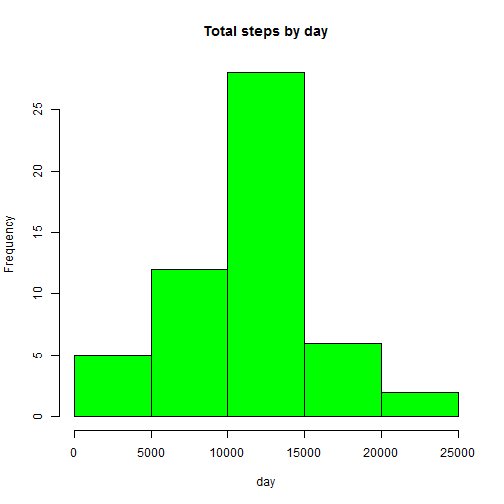
\includegraphics{PA1_template_files/figure-latex/unnamed-chunk-3-1.pdf}

\hypertarget{calculate-and-report-the-median-of-the-total-number-of-steps-taken-per-day}{%
\subsubsection{Calculate and report the median of the total number of
steps taken per
day}\label{calculate-and-report-the-median-of-the-total-number-of-steps-taken-per-day}}

\begin{Shaded}
\begin{Highlighting}[]
\NormalTok{medianSPD =}\StringTok{ }\KeywordTok{median}\NormalTok{(SPD}\OperatorTok{$}\NormalTok{steps)}
\NormalTok{medianSPD}
\end{Highlighting}
\end{Shaded}

\begin{verbatim}
## [1] 10765
\end{verbatim}

\hypertarget{calculate-and-report-the-mean-of-the-total-number-of-steps-taken-per-day}{%
\subsubsection{Calculate and report the mean of the total number of
steps taken per
day}\label{calculate-and-report-the-mean-of-the-total-number-of-steps-taken-per-day}}

\begin{Shaded}
\begin{Highlighting}[]
\NormalTok{meanSPD =}\StringTok{ }\KeywordTok{mean}\NormalTok{(SPD}\OperatorTok{$}\NormalTok{steps)}
\NormalTok{meanSPD}
\end{Highlighting}
\end{Shaded}

\begin{verbatim}
## [1] 10766.19
\end{verbatim}

\hypertarget{what-is-the-average-daily-activity-pattern}{%
\subsection{What is the average daily activity
pattern?}\label{what-is-the-average-daily-activity-pattern}}

\hypertarget{make-a-time-series-plot-of-the-5-minute-interval-x-axis-and-the-average-number-of-steps-taken-averaged-across-all-days-y-axis}{%
\subsubsection{Make a time series plot of the 5-minute interval (x-axis)
and the average number of steps taken, averaged across all days
(y-axis)}\label{make-a-time-series-plot-of-the-5-minute-interval-x-axis-and-the-average-number-of-steps-taken-averaged-across-all-days-y-axis}}

\begin{Shaded}
\begin{Highlighting}[]
\NormalTok{ASPI <-}\StringTok{ }\KeywordTok{aggregate}\NormalTok{(steps }\OperatorTok{~}\StringTok{ }\NormalTok{interval, activity, mean, }\DataTypeTok{na.rm=}\OtherTok{TRUE}\NormalTok{)}
\end{Highlighting}
\end{Shaded}

\begin{Shaded}
\begin{Highlighting}[]
\KeywordTok{ggplot}\NormalTok{(}\DataTypeTok{data =}\NormalTok{ ASPI)}\OperatorTok{+}
\StringTok{  }\KeywordTok{aes}\NormalTok{(}\DataTypeTok{x=}\NormalTok{interval,}\DataTypeTok{y=}\NormalTok{steps)}\OperatorTok{+}
\StringTok{  }\KeywordTok{geom_line}\NormalTok{()}\OperatorTok{+}
\StringTok{  }\KeywordTok{labs}\NormalTok{(}\DataTypeTok{title=} \StringTok{"Average Number of Steps Per Interval"}\NormalTok{)}
\end{Highlighting}
\end{Shaded}

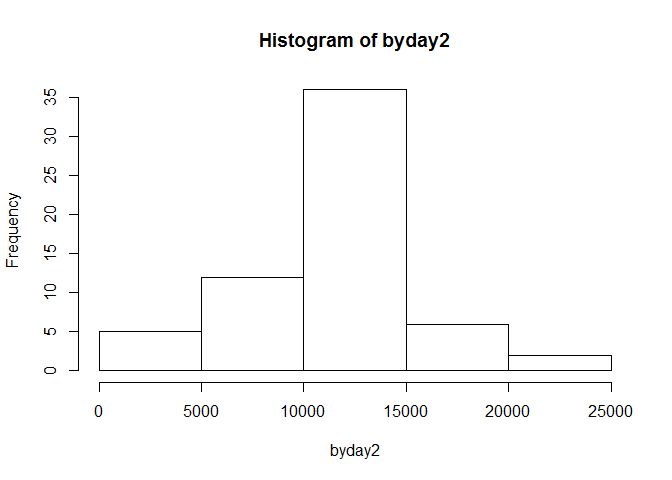
\includegraphics{PA1_template_files/figure-latex/unnamed-chunk-7-1.pdf}

\hypertarget{which-5-minute-interval-on-average-across-all-the-days-in-the-dataset-contains-the-maximum-number-of-steps}{%
\subsubsection{Which 5-minute interval, on average across all the days
in the dataset, contains the maximum number of
steps?}\label{which-5-minute-interval-on-average-across-all-the-days-in-the-dataset-contains-the-maximum-number-of-steps}}

\begin{Shaded}
\begin{Highlighting}[]
\NormalTok{result1 <-}
\StringTok{  }\NormalTok{ASPI }\OperatorTok
\StringTok{  }\KeywordTok{summarize}\NormalTok{(}\DataTypeTok{mInterval =} \KeywordTok{n}\NormalTok{(),}
            \DataTypeTok{msteps =} \KeywordTok{max}\NormalTok{(steps))}
  \KeywordTok{print}\NormalTok{(result1)}
\end{Highlighting}
\end{Shaded}

\begin{verbatim}
##   mInterval   msteps
## 1       288 206.1698
\end{verbatim}

\hypertarget{imputing-missing-values}{%
\subsection{Imputing missing values}\label{imputing-missing-values}}

\hypertarget{calculate-and-report-the-total-number-of-missing-values-in-the-dataset-i.e.-the-total-number-of-rows-with-nas}{%
\subsubsection{Calculate and report the total number of missing values
in the dataset (i.e.~the total number of rows with
NAs)}\label{calculate-and-report-the-total-number-of-missing-values-in-the-dataset-i.e.-the-total-number-of-rows-with-nas}}

\begin{Shaded}
\begin{Highlighting}[]
\NormalTok{missing <-}\StringTok{ }\KeywordTok{sum}\NormalTok{(}\KeywordTok{is.na}\NormalTok{(activity))}
\KeywordTok{print}\NormalTok{(missing)}
\end{Highlighting}
\end{Shaded}

\begin{verbatim}
## [1] 2304
\end{verbatim}

\hypertarget{devise-a-strategy-for-filling-in-all-of-the-missing-values-in-the-dataset.-create-a-new-dataset-that-is-equal-to-the-original-dataset-but-with-the-missing-data-filled-in.}{%
\subsubsection{Devise a strategy for filling in all of the missing
values in the dataset. Create a new dataset that is equal to the
original dataset but with the missing data filled
in.}\label{devise-a-strategy-for-filling-in-all-of-the-missing-values-in-the-dataset.-create-a-new-dataset-that-is-equal-to-the-original-dataset-but-with-the-missing-data-filled-in.}}

\begin{Shaded}
\begin{Highlighting}[]
\NormalTok{activity}\OperatorTok{$}\NormalTok{steps <-}\StringTok{ }\KeywordTok{as.numeric}\NormalTok{(activity}\OperatorTok{$}\NormalTok{steps) }
\NormalTok{activity <-}\StringTok{ }\NormalTok{activity }\OperatorTok
\StringTok{        }\KeywordTok{mutate}\NormalTok{(}\DataTypeTok{steps =} \KeywordTok{replace}\NormalTok{(steps,}
                                \KeywordTok{is.na}\NormalTok{(steps),}
                                \KeywordTok{mean}\NormalTok{(steps, }\DataTypeTok{na.rm=}\OtherTok{TRUE}\NormalTok{)))       }
\KeywordTok{summary}\NormalTok{(activity)}
\end{Highlighting}
\end{Shaded}

\begin{verbatim}
##      steps            date              interval     
##  Min.   :  0.00   Length:17568       Min.   :   0.0  
##  1st Qu.:  0.00   Class :character   1st Qu.: 588.8  
##  Median :  0.00   Mode  :character   Median :1177.5  
##  Mean   : 37.38                      Mean   :1177.5  
##  3rd Qu.: 37.38                      3rd Qu.:1766.2  
##  Max.   :806.00                      Max.   :2355.0
\end{verbatim}

\hypertarget{make-a-histogram-of-the-total-number-of-steps-taken-each-day-and-calculate-and-report-the-mean-and-median-total-number-of-steps-taken-per-day.-do-these-values-differ-from-the-estimates-from-the-first-part-of-the-assignment-what-is-the-impact-of-imputing-missing-data-on-the-estimates-of-the-total-daily-number-of-steps}{%
\subsubsection{Make a histogram of the total number of steps taken each
day and Calculate and report the mean and median total number of steps
taken per day. Do these values differ from the estimates from the first
part of the assignment? What is the impact of imputing missing data on
the estimates of the total daily number of
steps?}\label{make-a-histogram-of-the-total-number-of-steps-taken-each-day-and-calculate-and-report-the-mean-and-median-total-number-of-steps-taken-per-day.-do-these-values-differ-from-the-estimates-from-the-first-part-of-the-assignment-what-is-the-impact-of-imputing-missing-data-on-the-estimates-of-the-total-daily-number-of-steps}}

\begin{Shaded}
\begin{Highlighting}[]
\NormalTok{SPD1 <-}\StringTok{ }\KeywordTok{aggregate}\NormalTok{(steps }\OperatorTok{~}\StringTok{ }\NormalTok{date, activity, sum)}
\end{Highlighting}
\end{Shaded}

\begin{Shaded}
\begin{Highlighting}[]
\KeywordTok{hist}\NormalTok{(SPD1}\OperatorTok{$}\NormalTok{steps, }\DataTypeTok{col=}\StringTok{"blue"}\NormalTok{)}
\KeywordTok{abline}\NormalTok{(}\DataTypeTok{v =} \KeywordTok{median}\NormalTok{(SPD}\OperatorTok{$}\NormalTok{steps), }\DataTypeTok{col =} \StringTok{"green"}\NormalTok{, }\DataTypeTok{lwd =} \DecValTok{4}\NormalTok{)}
\end{Highlighting}
\end{Shaded}

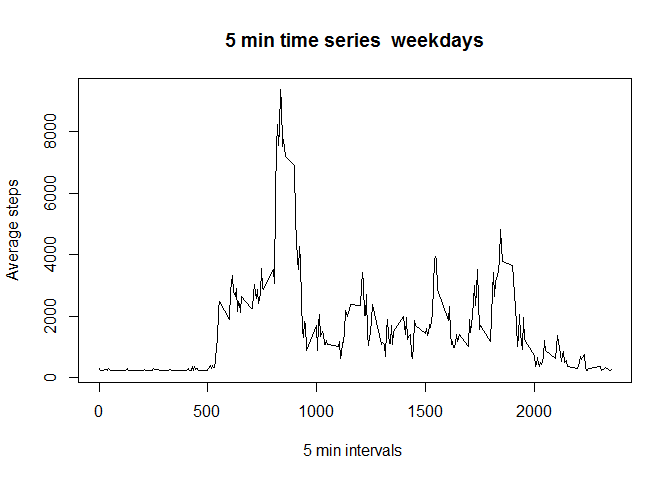
\includegraphics{PA1_template_files/figure-latex/unnamed-chunk-12-1.pdf}

\begin{Shaded}
\begin{Highlighting}[]
\NormalTok{medianSPD1 =}\StringTok{ }\KeywordTok{median}\NormalTok{(SPD1}\OperatorTok{$}\NormalTok{steps)}
\NormalTok{medianSPD1}
\end{Highlighting}
\end{Shaded}

\begin{verbatim}
## [1] 10766.19
\end{verbatim}

\begin{Shaded}
\begin{Highlighting}[]
\NormalTok{meanSPD1 =}\StringTok{ }\KeywordTok{mean}\NormalTok{(SPD1}\OperatorTok{$}\NormalTok{steps)}
\NormalTok{meanSPD1}
\end{Highlighting}
\end{Shaded}

\begin{verbatim}
## [1] 10766.19
\end{verbatim}

\begin{Shaded}
\begin{Highlighting}[]
\NormalTok{SummaryEstimates <-}\StringTok{ }\KeywordTok{cbind}\NormalTok{(medianSPD,medianSPD1, meanSPD, meanSPD1)}
\NormalTok{SummaryEstimates}
\end{Highlighting}
\end{Shaded}

\begin{verbatim}
##      medianSPD medianSPD1  meanSPD meanSPD1
## [1,]     10765   10766.19 10766.19 10766.19
\end{verbatim}

\hypertarget{are-there-differences-in-activity-patterns-between-weekdays-and-weekends}{%
\subsection{Are there differences in activity patterns between weekdays
and
weekends?}\label{are-there-differences-in-activity-patterns-between-weekdays-and-weekends}}

\hypertarget{create-a-new-factor-variable-in-the-dataset-with-two-levels-weekday-and-weekend-indicating-whether-a-given-date-is-a-weekday-or-weekend-day.}{%
\subsubsection{Create a new factor variable in the dataset with two
levels -- ``weekday'' and ``weekend'' indicating whether a given date is
a weekday or weekend
day.}\label{create-a-new-factor-variable-in-the-dataset-with-two-levels-weekday-and-weekend-indicating-whether-a-given-date-is-a-weekday-or-weekend-day.}}

\begin{Shaded}
\begin{Highlighting}[]
\NormalTok{activity}\OperatorTok{$}\NormalTok{date <-}\StringTok{ }\KeywordTok{as.Date}\NormalTok{(activity}\OperatorTok{$}\NormalTok{date)}
\NormalTok{weekdays1 <-}\StringTok{ }\KeywordTok{c}\NormalTok{(}\StringTok{'Monday'}\NormalTok{, }\StringTok{'Tuesday'}\NormalTok{, }\StringTok{'Wednesday'}\NormalTok{, }\StringTok{'Thursday'}\NormalTok{, }\StringTok{'Friday'}\NormalTok{)}
\NormalTok{activity}\OperatorTok{$}\NormalTok{wDay <-}\StringTok{ }\KeywordTok{factor}\NormalTok{((}\KeywordTok{weekdays}\NormalTok{(activity}\OperatorTok{$}\NormalTok{date) }\OperatorTok\StringTok{ }\NormalTok{weekdays1), }
         \DataTypeTok{levels=}\KeywordTok{c}\NormalTok{(}\OtherTok{FALSE}\NormalTok{, }\OtherTok{TRUE}\NormalTok{), }\DataTypeTok{labels=}\KeywordTok{c}\NormalTok{(}\StringTok{'weekend'}\NormalTok{, }\StringTok{'weekday'}\NormalTok{)) }
\end{Highlighting}
\end{Shaded}

\hypertarget{make-a-panel-plot-containing-a-time-series-plot-of-the-5-minute-interval-x-axis-and-the-average-number-of-steps-taken-averaged-across-all-weekday-days-or-weekend-days-y-axis.}{%
\subsubsection{Make a panel plot containing a time series plot of the
5-minute interval (x-axis) and the average number of steps taken,
averaged across all weekday days or weekend days
(y-axis).}\label{make-a-panel-plot-containing-a-time-series-plot-of-the-5-minute-interval-x-axis-and-the-average-number-of-steps-taken-averaged-across-all-weekday-days-or-weekend-days-y-axis.}}

\begin{Shaded}
\begin{Highlighting}[]
\NormalTok{ASPI1 <-}\StringTok{ }\KeywordTok{aggregate}\NormalTok{(steps }\OperatorTok{~}\StringTok{ }\NormalTok{interval }\OperatorTok{+}\StringTok{ }\NormalTok{wDay, activity, mean, }\DataTypeTok{na.rm=}\OtherTok{TRUE}\NormalTok{)}
\end{Highlighting}
\end{Shaded}

\begin{Shaded}
\begin{Highlighting}[]
\KeywordTok{ggplot}\NormalTok{(}\DataTypeTok{data =}\NormalTok{ ASPI1)}\OperatorTok{+}
\StringTok{  }\KeywordTok{aes}\NormalTok{(}\DataTypeTok{x=}\NormalTok{interval,}\DataTypeTok{y=}\NormalTok{ steps, }\DataTypeTok{group =}\NormalTok{ wDay, }\DataTypeTok{col =}\NormalTok{ wDay)}\OperatorTok{+}
\StringTok{  }\KeywordTok{geom_line}\NormalTok{()}\OperatorTok{+}
\StringTok{  }\KeywordTok{facet_grid}\NormalTok{(wDay}\OperatorTok{~}\NormalTok{.)}
\end{Highlighting}
\end{Shaded}

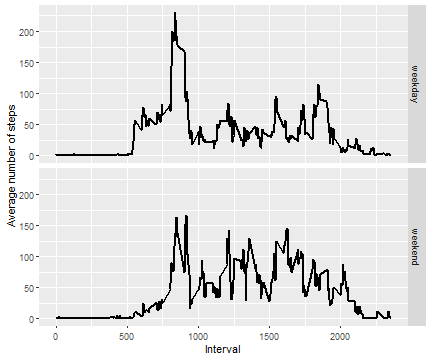
\includegraphics{PA1_template_files/figure-latex/unnamed-chunk-18-1.pdf}

\begin{Shaded}
\begin{Highlighting}[]
  \KeywordTok{labs}\NormalTok{(}\DataTypeTok{title=} \StringTok{"Average Steps Per Interval by Days"}\NormalTok{) }
\end{Highlighting}
\end{Shaded}

\begin{verbatim}
## $title
## [1] "Average Steps Per Interval by Days"
## 
## attr(,"class")
## [1] "labels"
\end{verbatim}

\end{document}
